%%%%%%%%%%%%%%%%%%%%%%%%%%%%%%%%%%%%%%%%%%%%%%%%%%%%%%%%%%%%%%%%
%%                                                            %%
%%   essentialsOfLatin, Italian translation 2017              %%
%%                                                            %%
%% From:  Henry C. Pearson, Essentials Of Latin For Beginners %%
%%        (1915, New York, American Book Company)             %%
%%                                                            %%
%%    https://archive.org/details/essentialslatin04peargoog   %%
%%                                                            %%
%% Translated by g.p.ciceri <gp.ciceri@gmail.com>             %%
%% ---------------------------------------------------------- %%
%% This translation is Licensed under                         %%
%% Creative Commons Attribution-ShareAlike 4.0 International  %%
%% https://creativecommons.org/licenses/by-sa/4.0/            %%
%%                                                            %%
%%%%%%%%%%%%%%%%%%%%%%%%%%%%%%%%%%%%%%%%%%%%%%%%%%%%%%%%%%%%%%%%

% āēīōū
% ăĕĭŏŭ




\documentclass[nols]{tufte-handout}

%\geometry{showframe} % display margins for debugging page layout

\usepackage{fontspec}
\usepackage{ifxetex}
\setmainfont[Path=./fonts/palatino-linotype/, ItalicFont=palai.ttf, BoldFont=palab.ttf]{pala.ttf}


% \defaultfontfeatures{Mapping=tex-text}
% \setromanfont[Path=./fonts/TeX-Gyre-Schola/,Mapping=tex-text]{TeX Gyre Schola}
% \setsansfont[Path=./fonts/TeX-Gyre-Heros/,Scale=MatchLowercase,Mapping=tex-text]{TeX Gyre Heros}
% \setmonofont[Path=./fonts/TeX-Gyre-Cursor/,Scale=MatchLowercase]{TeX Gyre Cursor}

\usepackage{lipsum}
\usepackage{url}
\usepackage{longtable}
\usepackage{stackengine}

\usepackage{graphicx} % allow embedded images
  \setkeys{Gin}{width=\linewidth,totalheight=\textheight,keepaspectratio}
  \graphicspath{{graphics/}} % set of paths to search for images
\usepackage{amsmath}  % extended mathematics
\usepackage{booktabs} % book-quality tables
\usepackage{units}    % non-stacked fractions and better unit spacing
\usepackage{multicol} % multiple column layout facilities
\usepackage{lipsum}   % filler text
\usepackage{fancyvrb} % extended verbatim environments
  \fvset{fontsize=\normalsize}% default font size for fancy-verbatim environments

% Standardize command font styles and environments
\newcommand{\doccmd}[1]{\texttt{\textbackslash#1}}% command name -- adds backslash automatically
\newcommand{\docopt}[1]{\ensuremath{\langle}\textrm{\textit{#1}}\ensuremath{\rangle}}% optional command argument
\newcommand{\docarg}[1]{\textrm{\textit{#1}}}% (required) command argument
\newcommand{\docenv}[1]{\textsf{#1}}% environment name
\newcommand{\docpkg}[1]{\texttt{#1}}% package name
\newcommand{\doccls}[1]{\texttt{#1}}% document class name
\newcommand{\docclsopt}[1]{\texttt{#1}}% document class option name
\newenvironment{docspec}{\begin{quote}\noindent}{\end{quote}}% command specification environment

% concetti morfosintattici
\usepackage{xspace} 
\newcommand{\noun}{\textsc{sostantivo}\xspace}
\newcommand{\nouns}{\textsc{sostantivi}\xspace}
\newcommand{\adject}{\textsc{aggettivo}\xspace}
\newcommand{\adjects}{\textsc{aggettivi}\xspace}
\newcommand{\gnumber}{\textsc{numero}\xspace}
\newcommand{\gnumbers}{\textsc{numeri}\xspace}
\newcommand{\gender}{\textsc{genere}\xspace}
\newcommand{\genders}{\textsc{generi}\xspace}
\newcommand{\gcase}{\textsc{caso}\xspace}
\newcommand{\gcases}{\textsc{casi}\xspace}
\newcommand{\tense}{\textsc{tempo}\xspace}
\newcommand{\mood}{\textsc{modo}\xspace}
\newcommand{\gverb}{\textsc{verbo}\xspace}
\newcommand{\gverbs}{\textsc{verbi}\xspace}
\newcommand{\adjective}{\textsc{aggettivo}\xspace}
\newcommand{\nom}{\textsc{nom}\xspace}
\newcommand{\gen}{\textsc{gen}\xspace}
\newcommand{\dat}{\textsc{dat}\xspace}
\newcommand{\acc}{\textsc{acc}\xspace}
\newcommand{\voc}{\textsc{voc}\xspace}
\newcommand{\abl}{\textsc{abl}\xspace}
\newcommand{\gexit}{\textsc{uscita}\xspace}
\newcommand{\gexits}{\textsc{uscite}\xspace}
\newcommand{\declinazione}{\textsc{declinazione}\xspace}
\newcommand{\masc}{\textsc{maschile}\xspace}
\newcommand{\femm}{\textsc{femminile}\xspace}
\newcommand{\neut}{\textsc{neutro}\xspace}

\newcommand{\indic}{\textsc{indicativo}\xspace}
\newcommand{\imper}{\textsc{imperativo}\xspace}
\newcommand{\gcong}{\textsc{congiuntivo}\xspace}
\newcommand{\ott}{\textsc{ottativo}\xspace}
\newcommand{\partic}{\textsc{participio}\xspace}
\newcommand{\infin}{\textsc{infinito}\xspace}

\newcommand{\pres}{\textsc{presente}\xspace}
\newcommand{\imperf}{\textsc{imperfetto}\xspace}
\newcommand{\aor}{\textsc{aoristo}\xspace}
\newcommand{\fut}{\textsc{futuro}\xspace}
\newcommand{\perf}{\textsc{perfetto}\xspace}
\newcommand{\pperf}{\textsc{piuccheperfetto}\xspace}

\newcommand{\sing}{\textsc{singolare}\xspace}
\newcommand{\plur}{\textsc{plurale}\xspace}
\newcommand{\dual}{\textsc{duale}\xspace}

\newcommand{\si}{\textsc{sing}\xspace}
\newcommand{\pl}{\textsc{plur}\xspace}
\newcommand{\du}{\textsc{dual}\xspace}

\newcommand{\att}{\textsc{attivo}\xspace}
\newcommand{\med}{\textsc{medio}\xspace}
\newcommand{\pass}{\textsc{passivo}\xspace}
\newcommand{\medpass}{\textsc{medio-passivo}\xspace}


% italianitudini
\renewcommand{\figurename}{Figura}
\renewcommand{\tablename}{Tabella}
\renewcommand{\contentsname}{Indice}

% fix per un qualche problema
\ifxetex
  \newcommand{\textls}[2][5]{%
    \begingroup\addfontfeatures{LetterSpace=#1}#2\endgroup
  }
  \renewcommand{\allcapsspacing}[1]{\textls[15]{#1}}
  \renewcommand{\smallcapsspacing}[1]{\textls[10]{#1}}
  \renewcommand{\allcaps}[1]{\textls[15]{\MakeTextUppercase{#1}}}
  \renewcommand{\smallcaps}[1]{\smallcapsspacing{\scshape\MakeTextLowercase{#1}}}
  \renewcommand{\textsc}[1]{\smallcapsspacing{\textsmallcaps{#1}}}
\fi

% too many float...
\extrafloats{100}
% āēīōū
% ăĕĭŏŭ

\title{Essentials Of Latin. Elementi di Latino. \newline Lezione XIV - Seconda Coniugazione. Caratteristiche. Coniugazione dell'Indicativo Attivo.}

\author[gpciceri]{a cura di Milagathòs: Milo's help to enjoy humanities.}

\date{27 Febbrajo 2017} % without \date command, current date is supplied


\begin{document}

\hyphenation{co-niu-ga-zio-ne}

\maketitle% this prints the handout title, author, and date

\begin{marginfigure}[-2.5cm]
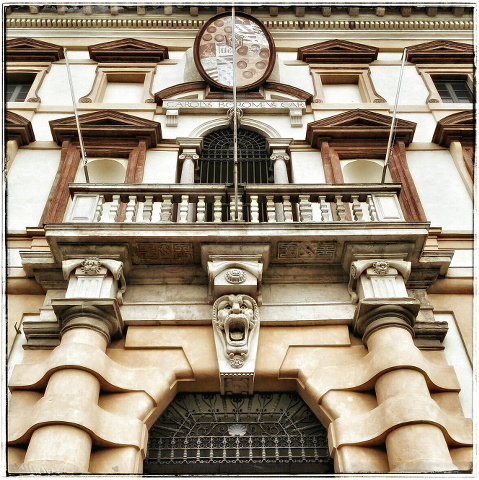
\includegraphics{smallthumb-lesson_I.jpeg}
\setfloatalignment{b}
\end{marginfigure}


\begin{abstract}
\noindent
Queste lezioni riprendono il testo introduttivo al Latino di Pearson\cite{pearson1915}, del quale seguono la numerazione; la struttura di ogni lezione è piuttosto regolare: inizia con \textsc{cenni di morfologia e di sintassi latina}, seguita da un \textsc{piccolo vocabolario} per il lessico; ci sono infine vari \textsc{esercizi} di traduzione e di composizione latina.

\bigskip
\noindent
Lezione XIV - Seconda coniugazione. Caratteristiche. Coniugazione dell'Indicativo Attivo. Vocabolario, esercizi.
\end{abstract}

%\printclassoptions

% āēīōū
% ăĕĭŏŭ

\newthought{104. Seconda Coniugazione.} Tutti i verbi il cui tema del presente termina in \textbf{ē} \textit{(e lunga)}
appartengono alla seconda coniugazione. I vari tempi di questi verbi sono formati a partire dalle parti principali,
proprio come per la prima coniugazione. Ripassa le sezioni (86.), (87.), (98.), (99.).

\newthought{Verbi Modello:} \textbf{moneō}, \textit{io ammonisco, consiglio}, \textbf{-es}, \textbf{monuī}, \textbf{monitum}, \textbf{monēre};
\textbf{videō}, \textit{io vedo, guardo}, \textbf{-es}, \textbf{vīdī}, \textbf{vīsum}, \textbf{vidēre}.


\begin{fullwidth}
\begin{table}[!htbp]
  \centering
  \begin{tabular}{l l l}
    %\toprule
	
	\multicolumn{3}{c}{\textsc{II Coniugazione, forme verbali dell'Indicativo Attivo}} \\
	
    \textsc{Presente} & mone\textbf{ō}, \textit{io ammonisco} & vide\textbf{ō}, \textit{io vedo}  \\
    \textsc{Imperfetto} & monē\textbf{bam}, \textit{io ammonivo} & vidē\textbf{bam}, \textit{io vedevo}   \\
    \textsc{Futuro} & monē\textbf{bō}, \textit{io ammonisco} & vidē\textbf{bō}, \textit{io vedrò}   \\
   
   \textsc{Perfetto} & monu\textbf{ī}, \textit{io ammonii} & vid\textbf{ī}, \textit{io vidi}   \\
   \textsc{Piuccheperfetto} & monu\textbf{eram}, \textit{io avevo ammonto} & vid\textbf{eram}, \textit{io avevo visto}    \\
   \textsc{Futuro Perfetto} & monu\textbf{erō}, \textit{io avrò ammonito} & vid\textbf{erō}, \textit{io avrò visto}    \\
   
    %\bottomrule
  \end{tabular}
  %\caption[bottom]{Seconda Coniugazione, Indicativo attivo.}
  \label{tab:normaltab}
  %\zsavepos{pos:normaltab}
\end{table}
\end{fullwidth}

\newthought{105. Seconda Coniugazione. Indicativo Presente Attivo}

\begin{fullwidth}
\begin{table}[!htbp]
  \centering
  \begin{tabular}{l l}
    %\toprule
	
	\multicolumn{2}{c}{\textsc{Coniugazione dell'Indicativo Presente Attivo} di \textbf{moneō}} \\
	
	& \multicolumn{1}{c}{\textsc{Singolare}} \\

    \textsc{1.} & mone\textbf{ō}, \textit{io ammonisco}   \\
    \textsc{2.} & monē\textbf{s}, \textit{tu ammonisci}  \\
    \textsc{3.} & mone\textbf{t}, \textit{egli ammonisce}   \\
   
	& \multicolumn{1}{c}{\textsc{Plurale}} \\
	
    \textsc{1.} & monē\textbf{mus}, \textit{noi ammoniamo}    \\
    \textsc{2.} & monē\textbf{tis}, \textit{voi ammonite}    \\
    \textsc{3.} & mone\textbf{nt}, \textit{essi ammoniscono}    \\
	
    %\bottomrule
  \end{tabular}
  %\caption[bottom]{Seconda Coniugazione, Presente.}
  \label{tab:normaltab}
  %\zsavepos{pos:normaltab}
\end{table}
\end{fullwidth}

\newthought{Osservazioni}
\begin{itemize}
\item[\textsc{1.}] La \textbf{-ē-} del tema del presente è mantenuta anche prima dell'uscita personale in \textbf{-ō} della prima persona singolare
(nella prima coniugazione invece, la vocale tematica \textbf{-ā-} cade davanti alla \textbf{-ō}). 
\item[\textsc{2.}] Qual è la vocale caratteristica prima delle uscite personali di \textbf{moneō}? Di \textbf{amō}? 
\end{itemize}


\newthought{106. Seconda Coniugazione. Indicativo Perfetto Attivo}

\begin{fullwidth}
\begin{table}[!htbp]
  \centering
  \begin{tabular}{l l}
    %\toprule
	
	\multicolumn{2}{c}{\textsc{Coniugazione dell'Indicativo Perfetto Attivo} di \textbf{moneō}} \\
	
	& \multicolumn{1}{c}{\textsc{Singolare}} \\

    \textsc{1.} & mònu\textbf{ī}, \textit{io ammonii, ho ammonito}   \\
    \textsc{2.} & monu\textbf{ìstī}, \textit{tu ammonisti, hai ammonito}  \\
    \textsc{3.} & mònu\textbf{it}, \textit{egli ammonì, ha ammonito}   \\
   
	& \multicolumn{1}{c}{\textsc{Plurale}} \\
	
    \textsc{1.} & monù\textbf{mus}, \textit{noi ammonimmo, abbiamo ammonito}    \\
    \textsc{2.} & monu\textbf{ìstis}, \textit{voi ammoniste, avete ammonito}    \\
    \textsc{3.} & monu\textbf{ērunt}, \textit{essi ammonirono, hanno ammonito}    \\
	
    %\bottomrule
  \end{tabular}
  %\caption[bottom]{Seconda Coniugazione, Perfetto.}
  \label{tab:normaltab}
  %\zsavepos{pos:normaltab}
\end{table}
\end{fullwidth}

\newthought{Osservazioni}
\begin{itemize}
\item[\textsc{1.}] Gli accenti delle forme verbali sono tipici, e le desinenze personali sono uguali a quelle del perfetto di \textbf{amō}.
Il tema del perfetto \textbf{monu-} non finisce in \textbf{v}, come in \textbf{amō, amāv-}
\end{itemize}

% āēīōū
% ăĕĭŏŭ


\newthought{107.} I vari tempi dei verbi della Seconda Coniugazione sono coniugati come i corrispondenti della prima coniugazione (eccetto quanto evidenziato in (105.) 1 e 2). Coniuga tutti i tempi dell'indicativo attivo dei seguenti verbi:


\begin{itemize}
\item \textbf{habeō, -es, habuī, habitum, habēre}, \textit{io ho, tengo}  
\item \textbf{videō, -es, vidī, vīsum, vidēre}, \textit{io vedo}  
\end{itemize}

% āēīōū
% ăĕĭŏŭ

\newthought{108. Vocabolario} 

\begin{multicols}{2}
	\noindent \hangindent=1em \textbf{moneō, -es, monuī, monitum, monēre}, v.tr., \textit{ammonire, mettere in guardia}.  \\
	\noindent \hangindent=1em \textbf{habeō, -es, habuī, habitum, habēre}, v.tr., \textit{avere, tenere}.  \\
	\noindent \hangindent=1em \textbf{videō, -es, vīdī, viitum, vidēre}, v.tr., \textit{vedere}.  \\
	\noindent \hangindent=1em \textbf{terreō, -es, terruī, territum, terrēre}, v.tr., \textit{atterrire, impaurire}.  \\
	\noindent \hangindent=1em \textbf{moveō, -es, mōvī, mōtum, movēre}, v.tr., \textit{muovere}, \textbf{castra movēre}, \textit{sciogliere l'accampamento}.  \\
	\noindent \hangindent=1em \textbf{dīmicō, -as, -āvī, -ātum, -āre}, v.intr., \textit{combattere, contendere}.  \\
	\noindent \hangindent=1em \textbf{praeda, -ae}, f., \textit{preda, spoglia}.  \\
    \noindent \hangindent=1em \textbf{perīculum, -ī}, n., \textit{pericolo}.  \\
	\noindent \hangindent=1em \textbf{cum}, prep. con \abl, \textit{con}.  \\
	
\end{multicols}
% āēīōū
% ăĕĭŏŭ

\newthought{109. Esercizi di Ripasso}
\\
\textsc{I.} \quad
\textsc{1.}~Saxis telis Galli cum Romanls pugnabant. \quad
\textsc{2.}~Magnum bellum contra Romanes paraverant. \quad
\textsc{3.}~Ad portam liberos portaverunt. \quad
\textsc{4.}~Paucos libros amico meo dedi. \quad
\textsc{5.}~Romani multa arma in hibema portabunt. \quad
\textsc{6.}~Cur oppidum expugnare maturaverunt?
\\
\textsc{II.} \quad
\textsc{1.}~Armarono i fieri abitanti con giavellotti. \quad
\textsc{2.}~Vicino all'accampamento vi erano poche costruzioni. \quad
\textsc{3.}~Non sempre occupiamo le città. \quad
\textsc{4.}~Hai dato un libro al mio amico?


\newthought{110. Esercizi}
\\
\textsc{I.} \quad
\textsc{1.}~Movebat; vidit; terruerat. \quad
\textsc{2.}~Viderimus; movisti; habebis. \quad
\textsc{3.}~Moverant; terruerunt; moverint. \quad
\textsc{4.}~Romani cum Helvetils dimicabant. \quad
\textsc{5.}~Periculum magnum oppidi incolas terruerat. \quad
\textsc{6.}~Praedam in vicis multam viderunt. \quad
\textsc{7.}~Galli copias ad oppidum moverant. \quad
\textsc{8.}~Vidistine tuum periculum ? \quad
\textsc{9.}~Pueri multa praemia habebunt. \quad
\textsc{10.}~Romani gladiis et pilis agricolas terruerunt. \quad
\textsc{11.}~Mox copiam frumenti habuerit. \quad
\textsc{12.}~Praeda nautas pigros delectabit. 
\\
II. I. She had seen; he has frightened; he will have 
had. 2. We had moved; you (plur.) have seen; they have 
fought. 3. The Gauls broke up camp. 4. They had con- 
tended with the inhabitants. 5. The messenger frightened 
the lieutenant by the story. 6. There is great danger in 
wine. 

\textsc{II.} \quad
\textsc{1.}~Aveva visto, ha impaurito; avrà avuto. \quad
\textsc{2.}~Aveva mosso; hai visto; combatterono. \quad
\textsc{3.}~I Galli sciolseto l'accampamento. \quad
\textsc{4.}~Avevano conteso con gli abitanti. \quad
\textsc{5.}~Il messaggero spaventò il luogotenente con la storia. \quad
\textsc{6.}~Vi è grande pericolo nel vino. 

\begin{figure}[!b]
  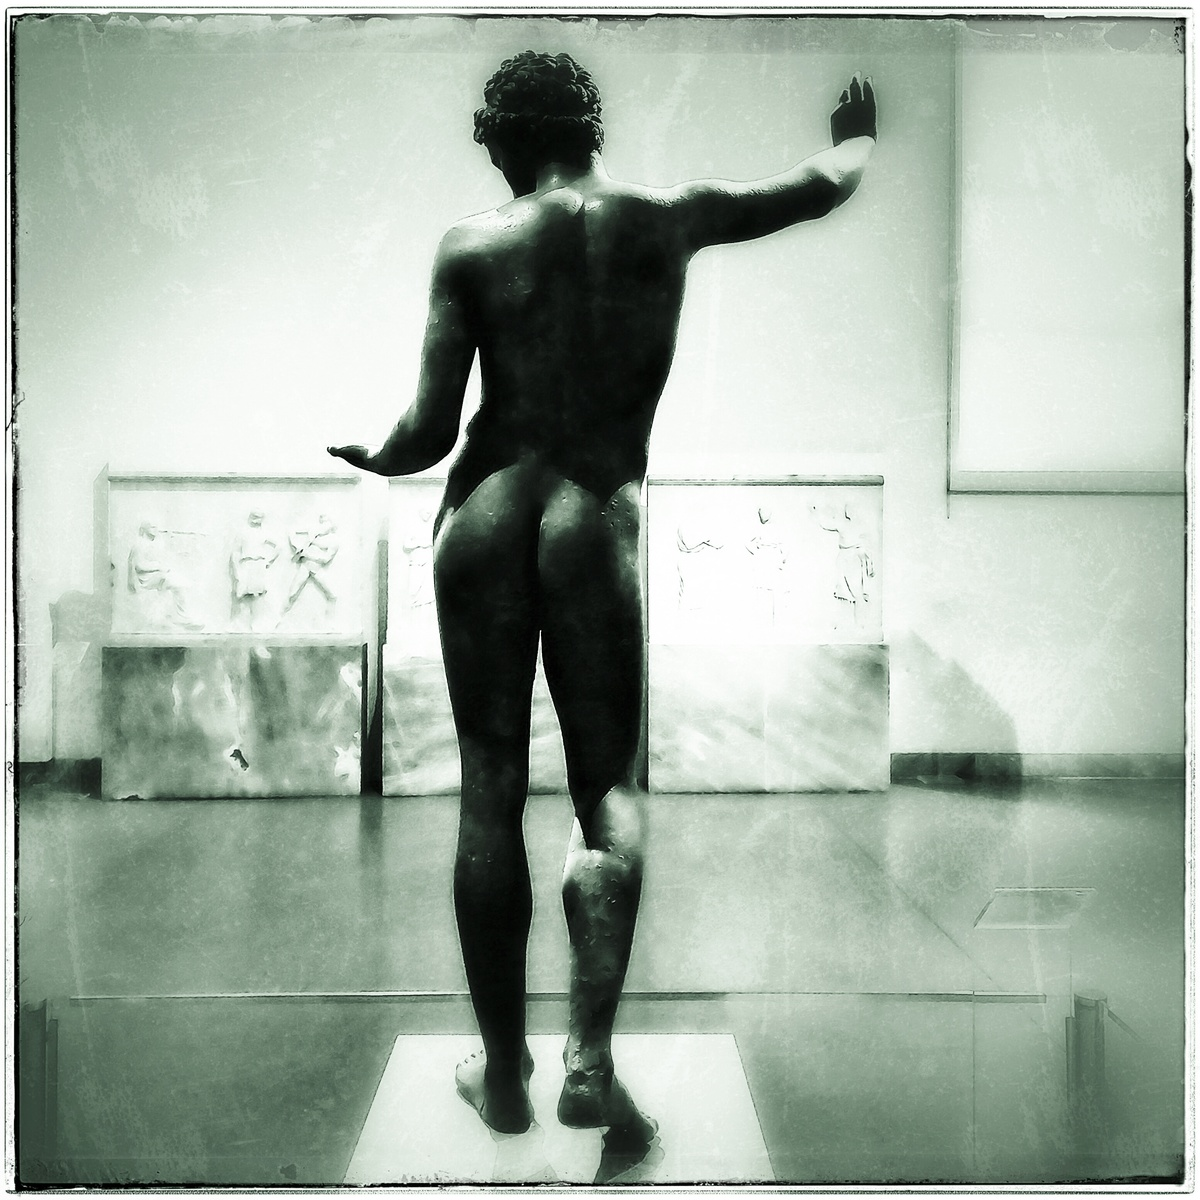
\includegraphics[width=0.8\linewidth]{thumb-lesson_VII.jpeg}
  %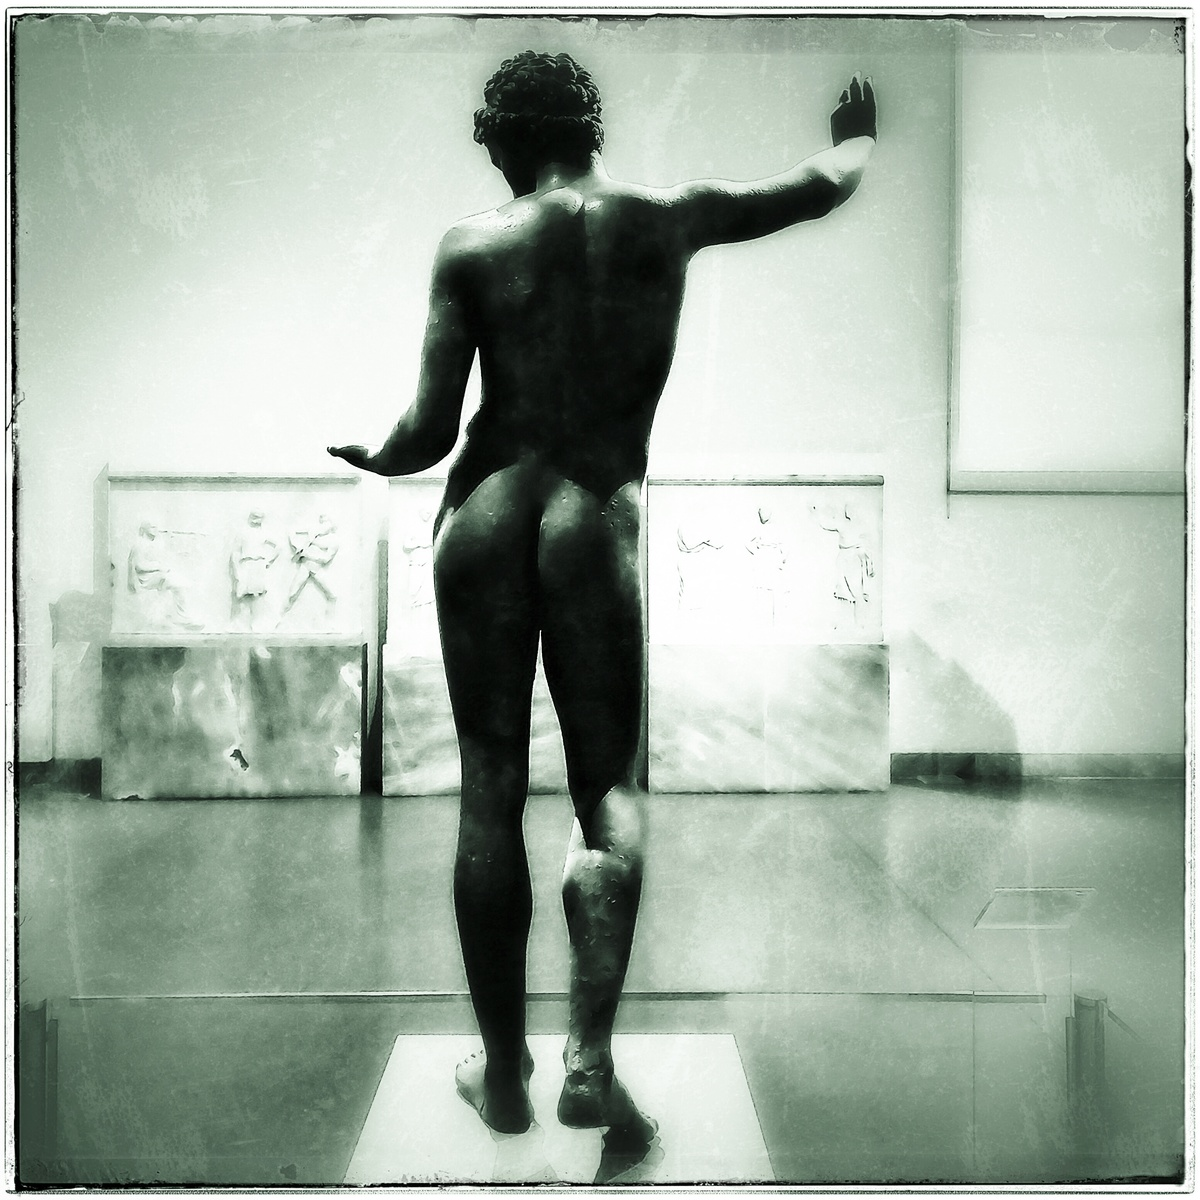
\includegraphics{thumb-lesson_VII.jpeg}
  \caption{Pavia: Almo Collegio Borromeo}
  \label{fig:textfig}
  %\zsavepos{pos:textfig}
  %\setfloatalignment{b}
\end{figure}

 

\nobibliography{latinBiblio}
\bibliographystyle{alpha}


\end{document}
